% ============================================================================
% Chuong: Danh gia va ket luan (BC2)
% ============================================================================

\chapter{ĐÁNH GIÁ VÀ KẾT LUẬN}
\label{ch:eval-bc2}
\label{ch:eval}

Chương này trình bày phương pháp và kết quả đánh giá định lượng hệ thống trên
một cụm Kubernetes thật, tập trung vào bốn câu hỏi: (i) hệ thống có phát hiện
đúng các hành vi quét cổng và dịch chuyển ngang hay không; (ii) tỷ lệ báo động
giả (\emph{false positive rate}, FPR) trên lưu lượng hợp lệ ở mức nào; (iii) chi
phí (\emph{overhead}) mà tầng thu thập eBPF áp lên nhân Linux là bao nhiêu; và
(iv) độ trễ của vòng phát hiện~$\rightarrow$~phản hồi. Toàn bộ số liệu trong
chương được đo bằng các kịch bản tự động (mục~\ref{sec:eval-method}), không phải
ước lượng lý thuyết.

\section{Phương pháp đánh giá}
\label{sec:eval-method}

\subsection{Môi trường thực nghiệm}

Thực nghiệm chạy trên một cụm Kubernetes thật gồm ba node (một node
control-plane và hai node worker), hệ điều hành Ubuntu~24.04, nhân Linux phiên
bản \texttt{6.8}, runtime container \texttt{containerd}, mạng pod do CNI
\emph{Calico} đảm nhiệm (hỗ trợ \texttt{NetworkPolicy}). Tầng thu thập là một
\texttt{DaemonSet} chạy chương trình eBPF \emph{CO-RE} gắn \texttt{kprobe} vào
hàm nhân \texttt{tcp\_v4\_connect}; mọi phép đo được thực hiện trên node
\texttt{worker-1}, nơi đặt các pod mục tiêu (dịch vụ \texttt{web} cổng~80 và
\texttt{api} cổng~8080).

\subsection{Bộ công cụ đo đạc}

Các kịch bản được đóng gói thành script có thể lặp lại
(thư mục \texttt{scripts/eval/} trong kho \texttt{K8sSecDaP-soc}):

\begin{itemize}[leftmargin=1.4em]
  \item \texttt{run-eval.sh} --- sinh các pod nguồn mới, chạy kịch bản tấn
        công/hợp lệ, kiểm tra cảnh báo tương ứng trong nhật ký pipeline eBPF,
        xuất bảng kết quả (Markdown + CSV).
  \item \texttt{overhead-ebpf.sh} và \texttt{overhead-repeat.sh} --- đo chi phí
        CPU nhân cho mỗi lời gọi \texttt{connect()} bằng cơ chế đếm thời gian
        chạy của chính nhân (\texttt{bpf\_stats}); bản \texttt{-repeat} lặp lại
        nhiều chu kỳ để tính khoảng tin cậy (mục~\ref{sec:eval-overhead}).
  \item \texttt{latency-report.sh} --- truy vấn cơ sở dữ liệu sự cố để tính độ
        trễ vòng phát hiện$\rightarrow$phản hồi (mục~\ref{sec:eval-latency}).
\end{itemize}

\subsection{Đặc tả bộ phát hiện đo được}

Qua khảo sát mã nguồn pipeline, luật phát hiện thực tế được xác định như sau:
một địa chỉ nguồn bị gắn cờ \texttt{port\_scan} khi \emph{số lượng kết nối} của
nó vượt ngưỡng $\tau = 40$ trong cửa sổ trượt kiểu \emph{tumbling} dài $60$~giây;
cảnh báo \texttt{blast\_radius} (dịch chuyển ngang) chỉ được tính cho nguồn đã
vượt ngưỡng đó và đo số pod mà nguồn tiếp cận được. Như vậy bộ phát hiện hoạt
động dựa trên \emph{tần suất kết nối theo nguồn}; đặc điểm này quyết định cách
thiết kế kịch bản hợp lệ ở mục~\ref{sec:eval-detect} và được phân tích kỹ ở
mục~\ref{sec:eval-limit}.

\subsection{Nguyên tắc tránh nhiễu thí nghiệm}

Vì bộ phát hiện khóa theo địa chỉ IP nguồn và IP của pod bị tái sử dụng nhanh,
một pod hợp lệ tạo ngay sau một pod quét có thể \emph{thừa hưởng} bộ đếm kết nối
của pod quét trong cùng cửa sổ 60~giây, gây dương tính giả \emph{giả tạo}. Để
loại bỏ hiện tượng này, harness (a)~chạy các mẫu hợp lệ \emph{trước} mọi kịch bản
tấn công, trên một cửa sổ đã được ``xả'' (chờ 75~giây), và (b)~cấp một pod nguồn
riêng cho mỗi mẫu. Đây là một bài học phương pháp luận quan trọng khi đánh giá
các bộ phát hiện khóa theo IP trong môi trường pod có vòng đời ngắn.

\section{Kết quả phát hiện và tỷ lệ báo động giả}
\label{sec:eval-detect}

Bảng~\ref{tab:eval-detect} tổng hợp kết quả. Bốn kịch bản tấn công đều được phát
hiện (\textbf{độ phủ phát hiện 4/4}); sáu mẫu lưu lượng hợp lệ với số kết nối từ
15 đến 38 (dưới ngưỡng) đều không sinh cảnh báo (\textbf{FPR $= 0/6$}). Hai mốc
biên xác nhận hiệu chỉnh ngưỡng: 38 kết nối không kích hoạt, 45 kết nối kích
hoạt --- khớp với ngưỡng $\tau = 40$. Kết quả nhất quán qua hai lần chạy độc lập.

\begin{table}[H]
  \centering
  \caption{Kết quả phát hiện trên cụm thật (node \texttt{worker-1}, nhân 6.8).
           Hai dòng cuối là minh hoạ giới hạn, không tính vào chỉ số chính.}
  \label{tab:eval-detect}
  \small
  \begin{tabularx}{\linewidth}{@{}l l l c@{}}
    \toprule
    \textbf{Kịch bản} & \textbf{Loại} & \textbf{Cảnh báo kỳ vọng} & \textbf{Kết quả} \\
    \midrule
    Quét dọc (1 đích, 200 cổng)      & tấn công & \texttt{port\_scan}    & Phát hiện \\
    Quét ngang (6 pod, 30 cổng)      & tấn công & \texttt{blast\_radius} & Phát hiện \\
    Quét dồn (1 đích, 1000 cổng)     & tấn công & \texttt{port\_scan}    & Phát hiện \\
    Biên trên (45 kết nối)           & tấn công & \texttt{port\_scan}    & Phát hiện \\
    \midrule
    Hợp lệ 15 kết nối                & hợp lệ   & (không)                & Không cảnh báo \\
    Hợp lệ 20 kết nối                & hợp lệ   & (không)                & Không cảnh báo \\
    Hợp lệ 25 kết nối                & hợp lệ   & (không)                & Không cảnh báo \\
    Hợp lệ 30 kết nối                & hợp lệ   & (không)                & Không cảnh báo \\
    Hợp lệ 35 kết nối                & hợp lệ   & (không)                & Không cảnh báo \\
    Biên dưới (38 kết nối)           & hợp lệ   & (không)                & Không cảnh báo \\
    \midrule
    \textit{Quét chậm (50 cổng, 2s/cổng)} & \textit{né tránh} & \texttt{port\_scan} & \textit{Bỏ sót (FN)} \\
    \textit{Hợp lệ ``ồn'' (60 kết nối)}   & \textit{giới hạn} & (không) & \textit{Báo giả (FP)} \\
    \bottomrule
  \end{tabularx}
\end{table}

\noindent\textbf{Độ phủ phát hiện:} 4/4 kịch bản tấn công.\quad
\textbf{Tỷ lệ báo động giả:} $0/6$ mẫu hợp lệ thực tế.

Hình~\ref{fig:eval-detection} trực quan hóa quá trình hiệu chỉnh quanh ngưỡng: sáu mẫu hợp
lệ (15--38 kết nối) đều nằm \emph{dưới} ngưỡng 40 nên không sinh cảnh báo, trong khi mẫu
tấn công ở biên (45 kết nối) vượt ngưỡng và bị bắt. Cột 60 kết nối là trường hợp giới hạn
``hợp lệ nhưng ồn'' --- một client hợp lệ tạo nhiều kết nối --- vượt ngưỡng và do đó bị báo
giả, minh họa đúng giới hạn của cách đếm theo \emph{khối lượng} kết nối đã phân tích ở
Chương~\ref{ch:foundations} (bộ đếm khóa theo địa chỉ nguồn).

\begin{figure}[H]
  \centering
  \resizebox{0.82\linewidth}{!}{% Bieu do hieu chinh phat hien: so ket noi/cua so vs nguong 40 (so lieu THAT). Chuong 5.
\begin{tikzpicture}
\begin{axis}[
    ybar,
    width=12cm, height=6.2cm,
    bar width=15pt,
    every axis plot/.append style={bar shift=0pt},
    ymin=0, ymax=70,
    ylabel={Số kết nối / cửa sổ 60\,s},
    xlabel={Mẫu đo (theo số kết nối)},
    xtick={1,2,3,4,5,6,7,8},
    xticklabels={15,20,25,30,35,38,45,60},
    enlarge x limits=0.08,
    nodes near coords, every node near coord/.append style={font=\scriptsize},
    tick label style={font=\scriptsize}, label style={font=\small},
    legend style={font=\scriptsize, at={(0.02,0.97)}, anchor=north west, draw=none, fill=none},
    legend cell align=left,
]
  \addplot[fill=blue!35, draw=blue!65] coordinates {(1,15)(2,20)(3,25)(4,30)(5,35)(6,38)};
  \addplot[fill=red!35,  draw=red!70]  coordinates {(7,45)(8,60)};
  \legend{hợp lệ --- không cảnh báo, $>$ ngưỡng --- cảnh báo}
  \draw[red!70!black, thick, dashed]
    (axis cs:0.4,40) -- (axis cs:8.6,40)
    node[below left=-2pt, font=\scriptsize]{ngưỡng = 40};
\end{axis}
\end{tikzpicture}
}
  \caption{Hiệu chỉnh ngưỡng phát hiện (số liệu đo thật).}
  \label{fig:eval-detection}
\end{figure}

Đáng chú ý là \emph{biên phân tách} quanh ngưỡng khá hẹp: mẫu hợp lệ cao nhất (38 kết
nối) và mẫu tấn công biên (45 kết nối) chỉ cách nhau $7$ kết nối, tức ngưỡng $\tau=40$
nằm gần như chính giữa. Biên hẹp này là hệ quả trực tiếp của việc đếm theo \emph{khối
lượng} kết nối: một client hợp lệ ``ồn'' và một cuộc quét ``nhẹ'' có thể tạo cùng một
lượng kết nối, nên không tồn tại một ngưỡng tĩnh nào tách sạch hai lớp. Quan sát này
củng cố cho hướng cải tiến đổi khóa đếm sang \emph{cặp (nguồn, cổng đích)} để đo số
cổng phân biệt~--~một đại lượng tách hai lớp tốt hơn~--~được phân tích ở
mục~\ref{sec:eval-limit}.

\section{Đánh giá hiệu năng}

\subsection{Chi phí CPU nhân của tầng eBPF}
\label{sec:eval-overhead}

Chi phí của hai chương trình eBPF (\texttt{kprobe} lúc vào và \texttt{kretprobe}
lúc ra của \texttt{tcp\_v4\_connect}) được đo bằng cơ chế \texttt{bpf\_stats} của
nhân: nhân tự ghi tổng thời gian chạy và số lần chạy của từng chương trình. Phép
đo lấy \emph{hiệu} của cặp giá trị này trước và sau một đợt tải kết nối, nên loại
được phần thời gian tích lũy trước khi bật bộ đếm; \texttt{bpftool} của host được
gọi qua \texttt{nsenter} từ chính pod thu thập (đặc quyền, \texttt{hostPID}) nên
\emph{không} cần gỡ bỏ collector và \emph{không} ảnh hưởng tới GitOps. Kết quả lấy
trung bình trên $n = 10$ chu kỳ, kèm khoảng tin cậy 95\% theo phân phối
Student-$t$ (Bảng~\ref{tab:eval-overhead}, Hình~\ref{fig:overhead-ebpf}).

\begin{table}[H]
  \centering
  \caption{Chi phí CPU nhân cho mỗi \texttt{connect()} (trung bình $\pm$ CI 95\%,
           $n = 10$ chu kỳ, $\approx$3000 kết nối/chu kỳ).}
  \label{tab:eval-overhead}
  \small
  \begin{tabular}{@{}l r@{}}
    \toprule
    \textbf{Chương trình eBPF} & \textbf{Chi phí / connect()} \\
    \midrule
    \texttt{kprobe} lúc vào (entry)        & $168 \pm 22$ ns \\
    \texttt{kretprobe} lúc ra (return)     & $1376 \pm 106$ ns \\
    \textbf{Tổng cộng mỗi connect()}       & $\mathbf{1544 \pm 126}$ \textbf{ns} \\
    \bottomrule
  \end{tabular}
\end{table}

\begin{figure}[H]
  \centering
  \resizebox{0.85\linewidth}{!}{%% Auto-generated by scripts/eval/overhead-repeat.sh -- eBPF per-connect overhead.
% Chi phi CPU kernel cho moi connect() (mean +/- 95% CI, n=10).
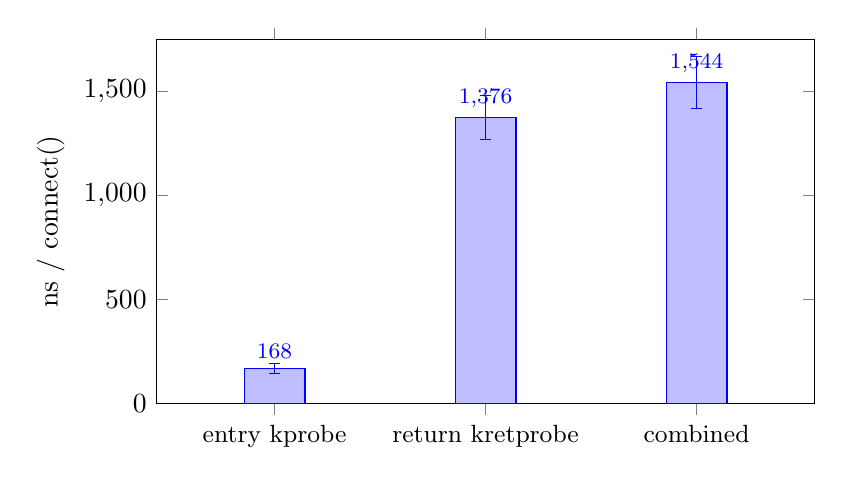
\begin{tikzpicture}
\begin{axis}[
    ybar, bar width=22pt, width=0.82\linewidth, height=6.2cm,
    ylabel={ns / connect()}, ymin=0, ymax=1750,
    symbolic x coords={entry kprobe, return kretprobe, combined},
    xtick=data, x tick label style={font=\small},
    nodes near coords, every node near coord/.append style={font=\footnotesize},
    error bars/y dir=both, error bars/y explicit,
    enlarge x limits=0.28,
]
\addplot+[fill=blue!25] coordinates {
    (entry kprobe,168) +- (0,22)
    (return kretprobe,1376) +- (0,106)
    (combined,1544) +- (0,126)
};
\end{axis}
\end{tikzpicture}
}
  \caption{Chi phí CPU nhân cho mỗi \texttt{connect()}.}
  \label{fig:overhead-ebpf}
\end{figure}

Phần lớn chi phí nằm ở nhánh trả về (\texttt{kretprobe}) do đây là nơi chương
trình dự trữ ô đệm vòng, tra cứu \texttt{LPM\_TRIE} phân loại CIDR và đẩy sự kiện
lên không gian người dùng. Quy đổi sang mức tải thực tế: ở $1000$ kết nối/giây,
tổng chi phí là $1544\,\text{ns} \times 1000 = 1{,}54\,\text{ms/giây}$, tức
$\approx 0{,}15\%$ một lõi CPU; ngay cả ở mức $3000$ kết nối/giây (đợt quét dồn)
cũng chỉ $\approx 0{,}46\%$ một lõi. Về phía không gian người dùng, tiến trình
collector chiếm $\approx 1$~mCPU và $3$~MiB bộ nhớ (mức sàn phân giải của
\texttt{kubectl top}), không đổi giữa lúc rảnh và lúc chịu tải. Như vậy tầng thu
thập eBPF có chi phí gần như không đáng kể, phù hợp với đặc tính của eBPF được
nêu trong tài liệu~\cite{gregg2019bpf}.

Từ chi phí đo được mỗi \texttt{connect()}, có thể \emph{suy diễn giải tích} mức tải mà
tầng eBPF chịu được trước khi chi phí trở nên đáng kể: Hình~\ref{fig:overhead-load}
chiếu tuyến tính con số $1544 \pm 126$~ns sang phần trăm một lõi CPU theo mức tải kết
nối. Đây là đường cong \emph{suy diễn} (không phải đo đa-mức-tải): vì mỗi
\texttt{connect()} đi qua đúng một lần cặp \texttt{kprobe}/\texttt{kretprobe}, tổng chi
phí tỉ lệ tuyến tính với số kết nối mỗi giây. Ngay ở mức $10\,000$ kết nối/giây~--~cao
hơn nhiều so với đợt quét dồn $\approx 3\,000$ quan sát được~--~chi phí cũng chỉ
$\approx 1{,}5\%$ một lõi. Việc \emph{đo thực nghiệm} đường cong này ở nhiều mức tải
trên cụm được để ở hướng phát triển (mục~\ref{sec:eval-limit}).

\begin{figure}[H]
  \centering
  \resizebox{0.82\linewidth}{!}{% Duong cong suy dien overhead-vs-tai: tu chi phi DO THAT 1544 ns/connect
% (Bang eval-overhead), chieu tuyen tinh sang % mot loi CPU theo connect/s.
% Day la SUY DIEN giai tich, KHONG phai do thuc nghiem da-muc-tai.
\begin{tikzpicture}
\begin{axis}[
    width=12cm, height=6.4cm,
    xlabel={Tải kết nối (connect/giây)},
    ylabel={Chi phí CPU nhân (\% một lõi)},
    xmin=0, xmax=10500, ymin=0, ymax=1.8,
    xtick={1000,2000,3000,5000,10000},
    xticklabels={1k,2k,3k,5k,10k},
    scaled x ticks=false,
    grid=both, grid style={gray!18},
    tick label style={font=\scriptsize}, label style={font=\small},
    legend style={font=\scriptsize, at={(0.02,0.97)}, anchor=north west, draw=none, fill=none},
    legend cell align=left,
]
  % Bien tren/duoi tu CI 95%: 1670 ns va 1418 ns / connect.
  \addplot[name path=hi, draw=none, forget plot] coordinates {(0,0)(1000,0.167)(2000,0.334)(3000,0.501)(5000,0.835)(10000,1.670)};
  \addplot[name path=lo, draw=none, forget plot] coordinates {(0,0)(1000,0.142)(2000,0.284)(3000,0.425)(5000,0.709)(10000,1.418)};
  \addplot[blue!12] fill between[of=hi and lo];
  \addlegendentry{khoảng CI 95\%}
  % Duong trung tam: 1544 ns/connect.
  \addplot[blue!70!black, very thick, mark=*, mark size=1.4pt]
    coordinates {(0,0)(1000,0.154)(2000,0.309)(3000,0.463)(5000,0.772)(10000,1.544)};
  \addlegendentry{$1544$ ns/connect (trung tâm)}
  % Moc tai thuc nghiem da quan sat.
  \draw[red!70!black, dashed] (axis cs:3000,0) -- (axis cs:3000,0.463)
    node[above left=-2pt, font=\scriptsize, text=red!70!black]{quét dồn $\approx$3k};
\end{axis}
\end{tikzpicture}
}
  \caption{Chi phí CPU nhân theo mức tải kết nối (suy diễn).}
  \label{fig:overhead-load}
\end{figure}

\subsection{Độ trễ vòng phát hiện $\rightarrow$ phản hồi}
\label{sec:eval-latency}

Độ trễ ``máy'' của SOC --- từ lúc nhận cảnh báo đến lúc áp \texttt{NetworkPolicy}
cách ly, \emph{không kể} thời gian con người duyệt --- có trung bình
$\approx 91$~ms, trung vị (p50) $54$~ms và phân vị 95 (p95) $234$~ms. Con số này
cho thấy một khi quyết định được duyệt, hệ thống chuyển từ cảnh báo sang thực thi
chính sách gần như tức thời; độ trễ tổng thể đầu-cuối bị chi phối bởi bước con
người trong vòng \emph{human-in-the-loop}, đúng như thiết kế.
Hình~\ref{fig:latency-pct} trực quan hóa ba mốc thống kê này. Khoảng cách giữa trung
vị ($54$~ms) và p95 ($234$~ms) phản ánh \emph{đuôi phân phối} dài~--~điển hình cho các
hệ phân tán trải qua tranh chấp lập lịch hoặc trễ mạng nội cụm ở một số ít sự cố~--~chứ
không phải mức trễ thường gặp. Việc dựng \emph{histogram/CDF} đầy đủ của phân phối độ
trễ đòi hỏi thu nhiều mẫu sự cố hơn trên cụm và được để ở hướng phát triển; ở đây báo
cáo chỉ trình bày các phân vị đã đo được, không nội suy phân phối.

\begin{figure}[H]
  \centering
  \resizebox{0.62\linewidth}{!}{% Do tre "may" cua vong phat hien -> ap NetworkPolicy (KHONG ke thoi gian con
% nguoi duyet). So lieu DO THAT tu latency-report.sh: p50=54, trung binh=91, p95=234 ms.
\begin{tikzpicture}
\begin{axis}[
    ybar,
    width=10cm, height=6cm,
    bar width=34pt,
    enlarge x limits=0.32,
    ymin=0, ymax=270,
    ylabel={Độ trễ máy (ms)},
    symbolic x coords={p50, trung bình, p95},
    xtick=data,
    nodes near coords, every node near coord/.append style={font=\small},
    tick label style={font=\small}, label style={font=\small},
]
  \addplot[fill=teal!45, draw=teal!70!black] coordinates {(p50,54) (trung bình,91) (p95,234)};
\end{axis}
\end{tikzpicture}
}
  \caption{Độ trễ máy của vòng phản hồi.}
  \label{fig:latency-pct}
\end{figure}

\section{So sánh với các công cụ liên quan}
\label{sec:eval-related}

Bảng~\ref{tab:eval-related} đối chiếu hệ thống của đồ án với bốn công cụ an ninh
runtime tiêu biểu cho Kubernetes. Điểm chung là đều khai thác eBPF/LSM để quan sát
ở kernel-space; điểm khác biệt nằm ở trọng tâm: các công cụ công nghiệp thiên về
quy tắc trên syscall (Falco~\cite{falco2024}) hoặc thực thi tổng quát
(Tetragon~\cite{tetragon2024}, KubeArmor~\cite{kubearmor2024},
Cilium~\cite{cilium2024}), trong khi hệ thống của đồ án tập trung hẹp vào bài toán
quét cổng/dịch chuyển ngang và \emph{lượng hoá} bằng cấu trúc dữ liệu luồng
(Count-Min Sketch, Tarjan, BFS) --- đây là đóng góp mang tính học thuật mà các
công cụ trên không đặt làm trọng tâm.

\begin{table}[H]
  \centering
  \caption{So sánh định tính với các công cụ an ninh runtime cho Kubernetes.}
  \label{tab:eval-related}
  \small
  \begin{tabularx}{\linewidth}{@{}l l X@{}}
    \toprule
    \textbf{Công cụ} & \textbf{Cơ chế nhân} & \textbf{Trọng tâm / khác biệt so với đồ án} \\
    \midrule
    Falco~\cite{falco2024}        & eBPF trên syscall   & Phát hiện theo \emph{luật} trên syscall; không có cấu trúc luồng lượng hoá quét cổng \\
    Tetragon~\cite{tetragon2024}  & eBPF (tracepoint/LSM) & Mạnh về \emph{thực thi} (kill/override) kernel-space; ít phân tích đồ thị dịch chuyển ngang \\
    Cilium~\cite{cilium2024}      & eBPF datapath (CNI) & Thực thi NetworkPolicy L3--L7 trong datapath; là tầng \emph{mạng}, không phải bộ phát hiện chuyên biệt \\
    KubeArmor~\cite{kubearmor2024}& BPF-LSM             & Thực thi chính sách hành vi process/file/network; không nhắm bài toán quét cổng \\
    \textbf{Đồ án này}            & eBPF \texttt{kprobe} & Phát hiện quét cổng/dịch chuyển ngang bằng \emph{cấu trúc dữ liệu luồng} + phản hồi NetworkPolicy có người duyệt \\
    \bottomrule
  \end{tabularx}
\end{table}

\section{Mô hình tin cậy và giới hạn an ninh của bộ thu thập}
\label{sec:eval-trust}

Vì bộ thu thập chạy dưới dạng \texttt{DaemonSet} đặc quyền và nạp mã eBPF vào nhân của
mỗi node, tôi xem nó là thành phần có quyền cao hơn hẳn ứng dụng thường và đặt nó vào
một ranh giới tin cậy riêng. Mục này phân tích mô hình tin cậy đó cùng các giới hạn an
ninh kèm theo, vì chính việc can thiệp vào không gian nhân đặt ra câu hỏi: nếu một pod
bị tấn công thì sao?

\textbf{Phân tách quyền theo pod.} Quyền đặc quyền nằm ở \emph{pod thu thập}, không ở
mọi pod ứng dụng. Nếu một pod ứng dụng bị chiếm, kẻ tấn công chỉ tạo được lưu lượng xấu
(quét cổng, dịch chuyển ngang)~--~tức làm \emph{tăng} khả năng bị hệ thống phát
hiện~--~chứ không tự có quyền chạm vào không gian nhân: chương trình eBPF đã được tôi
viết sẵn và gắn từ bộ thu thập, còn logic ở nhân chỉ \emph{nhận} sự kiện theo luồng
\texttt{connect()} (Mã nguồn~\ref{lst:bpf-kretprobe}, Chương~\ref{ch:impl}), không nhận
lệnh từ pod ứng dụng. Như vậy chiếm một pod ứng dụng làm tăng xác suất bị phát hiện,
không biến thành quyền điều khiển cảm biến.

\textbf{Ranh giới tin cậy thật sự.} Rủi ro đáng kể hơn là khi kẻ tấn công chiếm được
chính pod thu thập hoặc thoát ra node; khi đó họ có thể tác động đến cảm biến ở mức
nhân. Vì vậy tôi coi bộ thu thập là một \emph{trust boundary} riêng, không cùng mức tin
cậy với workload thường, và chủ trương làm cứng theo nguyên tắc đặc quyền tối thiểu:
chạy trên node pool riêng tách khỏi workload nhạy cảm; dùng ảnh bất biến, ký số, chỉ
cập nhật qua GitOps/CI; thay \texttt{privileged: true} bằng tập \emph{capability} tối
thiểu (\texttt{BPF}, \texttt{PERFMON}, \texttt{NET\_ADMIN}), gắn BTF chỉ đọc và bật
\texttt{readOnlyRootFilesystem}; không expose service và không cấp token RBAC rộng cho
pod thu thập, kèm profile \texttt{seccomp}/AppArmor.

\textbf{Đối chứng trong cùng pod.} Tôi đã áp nguyên tắc này ngay trong chính
\texttt{DaemonSet}: trong khi \texttt{collector} buộc phải đặc quyền, container sidecar
\texttt{alert-bridge} cạnh nó chạy theo chuẩn an toàn (\texttt{runAsNonRoot},
\texttt{readOnlyRootFilesystem}, \texttt{allowPrivilegeEscalation: false},
\texttt{capabilities.drop:[ALL]}) vì nó chỉ đọc tệp cảnh báo và đẩy lên NATS. Đây là
mẫu hình ``đặc quyền tối thiểu theo từng container'': chỉ thành phần thật sự cần chạm
nhân mới được cấp quyền cao.

\textbf{Giới hạn an ninh chưa khắc phục.} Tôi thừa nhận một điểm chưa hoàn thiện: bộ thu
thập hiện vẫn chạy \texttt{privileged: true} thay vì tập \emph{capability} tối thiểu nói
trên~--~manifest đã ghi chú hướng siết nhưng tôi chưa hiện thực. Đây là việc cần làm
trước khi đưa hệ thống vào môi trường sản xuất, và tôi xếp nó vào hướng phát triển.

\section{Giới hạn và hướng phát triển}
\label{sec:eval-limit}

Tôi ghi nhận thẳng thắn các giới hạn sau của hệ thống, kèm hướng khắc phục:

\begin{itemize}[leftmargin=1.4em]
  \item \textbf{Điểm mù cửa sổ tumbling (né tránh).} Một cuộc quét \emph{chậm}
        giữ số kết nối dưới ngưỡng trong mỗi cửa sổ 60~giây sẽ không bị phát hiện
        (dòng ``quét chậm'' trong Bảng~\ref{tab:eval-detect}). Hướng khắc phục:
        thay cửa sổ tumbling bằng \emph{sliding-window} CMS để bắt các luồng vắt
        biên cửa sổ.
  \item \textbf{Phát hiện theo lượng kết nối, không theo số cổng phân biệt
        (báo giả).} Vì bộ đếm khóa theo IP nguồn và cộng dồn \emph{mọi} kết nối,
        một client hợp lệ nhưng ``ồn'' (vượt 40 kết nối/cửa sổ tới ít cổng) vẫn bị
        gắn cờ (dòng ``hợp lệ ồn''). Hướng khắc phục: đổi khóa CMS sang
        \emph{cặp} (nguồn, cổng đích) để đếm \emph{số cổng phân biệt} --- đúng bản
        chất của hành vi quét cổng.
  \item \textbf{Phạm vi quan sát của \texttt{kprobe}.} \texttt{kprobe} trên
        \texttt{tcp\_v4\_connect} chỉ bắt lời gọi \texttt{connect()}, nên quét
        kiểu raw-SYN (\texttt{nmap -sS} với quyền root) đi vòng qua được; cần
        \texttt{-sT} (connect scan) để nằm trong tầm quan sát. Mở rộng sang
        \texttt{XDP}/\texttt{tc} sẽ bao phủ cả raw-SYN.
  \item \textbf{Phạm vi giao thức và quy mô.} Hiện chỉ hỗ trợ IPv4
        (\texttt{tcp\_v4\_connect}); ngưỡng $\tau$ là hằng số tĩnh, chưa thích
        nghi theo đặc tính tải; số liệu đo trên một node, chưa hợp nhất sketch đa
        node.
\end{itemize}

\subsection{Khó khăn triển khai và bài học rút ra}
\label{subsec:eval-lessons}

Bên cạnh các giới hạn về mặt thuật toán ở trên, quá trình triển khai trên cụm thật để
lại một số bài học mà tôi ghi lại trung thực, vì chúng định hình các quyết định kỹ
thuật của đồ án:

\begin{itemize}[leftmargin=1.4em]
  \item \textbf{Đổi CNI từ Flannel sang Calico để thực thi được chính sách.} Ban đầu
        tôi chọn Flannel vì nhẹ và dễ cài, nhưng khi kiểm thử bước phản hồi thì phát
        hiện \texttt{NetworkPolicy} cách ly \emph{không có tác dụng}: Flannel chỉ làm
        mạng overlay, không thực thi \texttt{NetworkPolicy}. Tôi phải chuyển CNI sang
        Calico (Tigera Operator) để có khả năng thực thi chính sách L3/L4~--~đây là lý
        do toàn bộ đánh giá được thực hiện trên Calico. Bài học: với bài toán
        \emph{ngăn chặn}, việc chọn CNI có thực thi chính sách là điều kiện tiên quyết,
        không phải lựa chọn tối ưu hóa.
  \item \textbf{Ngữ nghĩa cộng dồn của \texttt{NetworkPolicy}.} Bản nháp cách ly đầu
        tiên tôi sinh ra theo kiểu ``cho phép mọi nguồn \emph{trừ} kẻ tấn công'' ở
        chiều vào; khi kiểm thử mới thấy nó bị một luật cho-phép rộng khác vô hiệu hóa,
        vì \texttt{NetworkPolicy} mang ngữ nghĩa \emph{cộng dồn}. Tôi đổi sang
        \emph{chặn toàn bộ chiều ra của chính pod tấn công} (egress-deny), cách này
        không policy nào ghi đè được (Chương~\ref{ch:impl}).
  \item \textbf{Nhiễu do vòng đời pod ngắn.} Vì bộ phát hiện khóa theo IP nguồn mà IP
        pod bị tái sử dụng nhanh, một pod hợp lệ tạo ngay sau một pod quét có thể
        \emph{thừa hưởng} bộ đếm của pod quét trong cùng cửa sổ, gây dương tính giả giả
        tạo. Tôi khắc phục bằng cách chạy mẫu hợp lệ trên cửa sổ đã ``xả'' và cấp pod
        nguồn riêng cho mỗi mẫu (mục~\ref{sec:eval-method}).
  \item \textbf{Khác miền đồng hồ khi đo độ trễ.} Sự kiện eBPF mang mốc thời gian
        \emph{đồng hồ đơn điệu} của nhân (\texttt{bpf\_ktime\_get\_ns}), trong khi SOC
        ghi nhận theo \emph{đồng hồ tường}; hai miền không trừ trực tiếp được. Do đó
        tôi chỉ đo độ trễ ``máy'' phía SOC (mục~\ref{sec:eval-latency}) thay vì độ trễ
        đầu-cuối xuyên miền đồng hồ.
  \item \textbf{Đo chi phí nhân mà không phá vỡ GitOps.} Để đo chi phí eBPF, thay vì gỡ
        bộ thu thập (sẽ bị ArgoCD tự khôi phục), tôi bật \texttt{bpf\_stats} của nhân và
        lấy \emph{hiệu} số đếm trước/sau một đợt tải qua \texttt{bpftool} của host~--~đo
        tại chỗ, không can thiệp vào vòng đồng bộ (mục~\ref{sec:eval-overhead}).
  \item \textbf{Hai đường dữ liệu quan trắc dễ gây hiểu nhầm.} Console/Reports đọc trực
        tiếp PostgreSQL nên luôn đầy đủ sự cố tích lũy, trong khi dashboard Grafana lại
        thường \emph{trống}. Truy nguyên cho thấy đó là hai nguồn khác nhau: bảng
        \emph{Alerts Overview} đọc nhật ký Loki theo cửa sổ mặc định $30$~phút (không có
        tấn công gần đây thì trống), còn bảng \emph{Incidents \& Actions} đọc bộ đếm
        Prometheus vốn \emph{không được thu thập}~--~vì cụm dùng Prometheus Operator khám
        phá mục tiêu qua \texttt{ServiceMonitor} chứ không theo chú thích
        \texttt{prometheus.io/scrape}, và các bộ đếm còn bị đặt lại $0$ mỗi lần pod khởi
        động lại. Bài học: tách bạch rõ \emph{hệ thống ghi nhận bền vững} (cơ sở dữ liệu)
        với \emph{lớp quan trắc theo cửa sổ} (Grafana); cách bổ sung \texttt{ServiceMonitor}
        và nới cửa sổ thời gian để dashboard hiển thị đúng được nêu ở
        Phụ lục~\ref{app:demo-grafana}.
\end{itemize}

\section{Kết luận}

Đồ án đã hiện thực và \emph{kiểm chứng trên cụm Kubernetes thật} một hệ thống
phát hiện và ngăn chặn hành vi quét cổng/dịch chuyển ngang dựa trên eBPF kết hợp
cấu trúc dữ liệu luồng. Trên trục phát hiện, hệ thống đạt độ phủ 4/4 và FPR $0/6$
trên các mẫu hợp lệ thực tế, với ngưỡng được hiệu chỉnh rõ ràng. Trên trục hiệu
năng, tầng thu thập eBPF chỉ tốn $\approx 1544$~ns CPU nhân mỗi \texttt{connect()}
(dưới $0{,}5\%$ một lõi ngay cả khi chịu tải quét), và vòng phản hồi máy đạt p95
$234$~ms. Các giới hạn được nhận diện và đo lường tường minh (né tránh cửa sổ,
báo giả theo lượng kết nối) cùng hướng phát triển cụ thể (sliding-window CMS,
đổi khóa đếm theo cổng phân biệt, mở rộng XDP/\texttt{tc} và IPv6) tạo nền cho các
bước tiếp theo.
